\chapter{2010:Daniel Spielman}
\label{chap:spielman}
\begin{center}
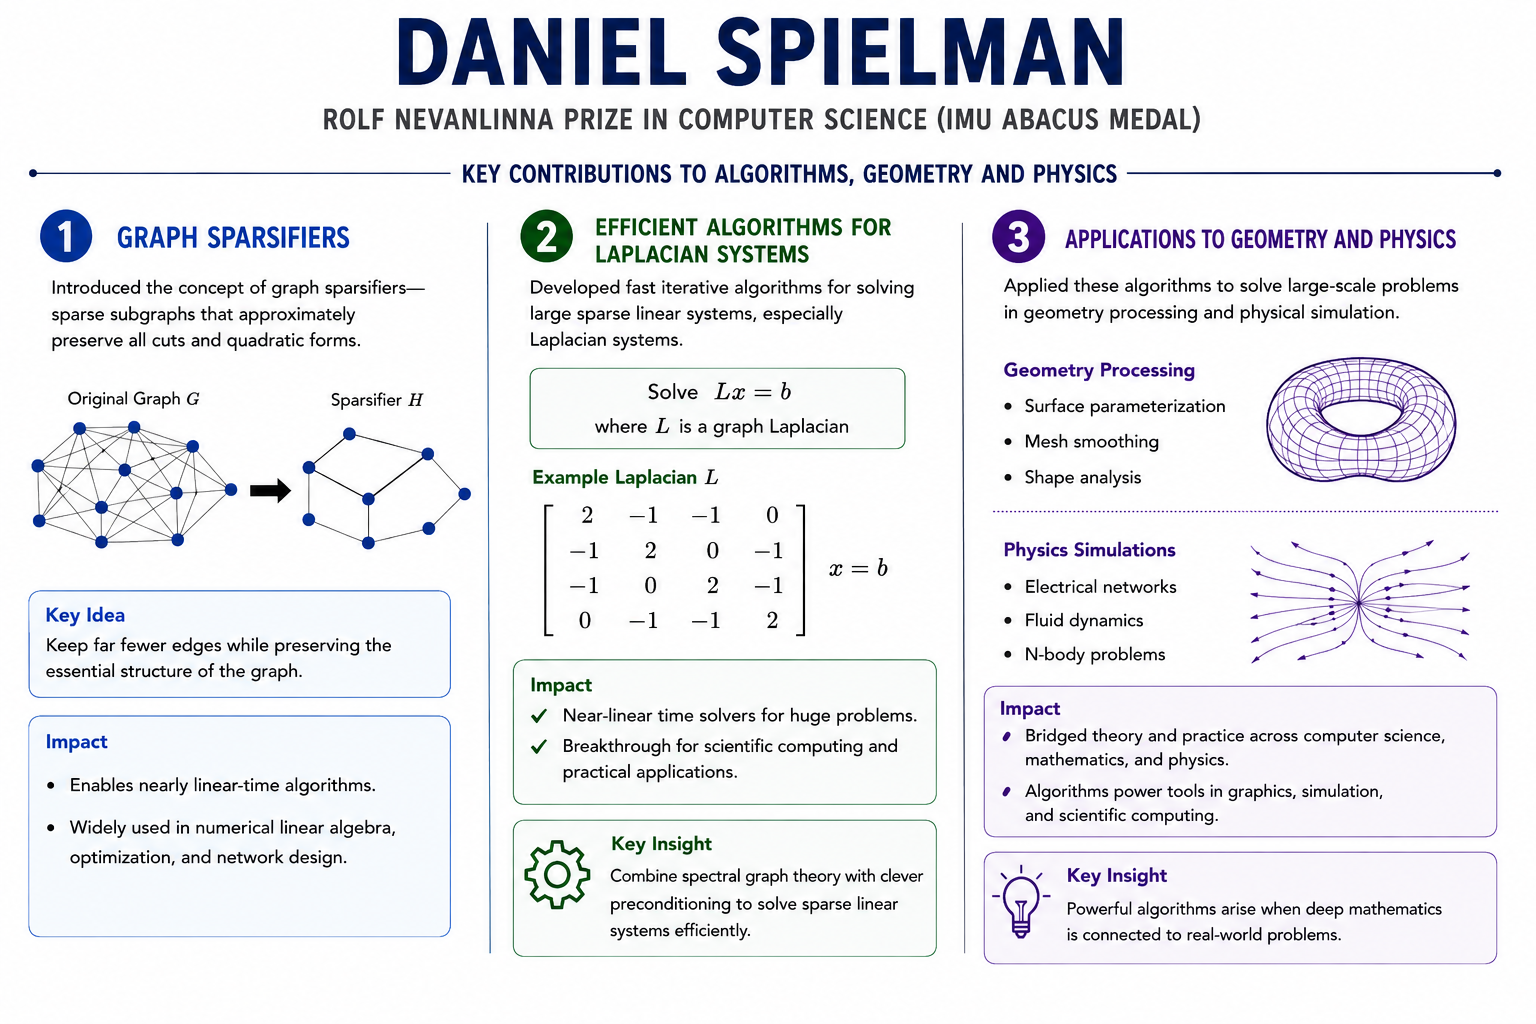
\includegraphics[width=\textwidth]{infographics/abacus8.png}
\end{center}
\targetchapterspacing
\index{Spielman, Daniel}
\booknote{The central habit in this chapter is to translate a network into a matrix and to demand of every approximation one thing: it must preserve the energy geometry of the original graph.}

\section{An Opening Story: Springs on a Water Line}

Three buildings stand in a row, each pair of neighbours joined by a pipe. Pipes resist differences: neighbours with pressures $u$ and $v$ stretch a pipe by $(u-v)^2$. For pressures $2$, $0$, $-1$, the pipes stretch by $(2-0)^2=4$ and $(0-(-1))^2=1$, total tension $5$: every assignment of pressures carries one number, the network's total tension.

Two questions seem far apart. \emph{Where is the weak joint?} A strong cluster meeting another across one rusty pipe lets pressures change on either side while tension stays small---the network is nearly two pieces. \emph{What pressures does the network settle at?} One linked equation per building; for a city, a huge system. Daniel Spielman's 2010 Rolf Nevanlinna Prize recognized that both are the same information read two ways, and that a matrix is the bookkeeping making the connection visible.

\section{The Problem}
Three problems about big networks, all questions a computer must answer quickly.

\noindent\textbf{Solving huge sparse systems.} Physical simulations produce one equation per point, coupling each point to its neighbours. A million-point mesh gives $Lx=b$ with a million unknowns and a handful of nonzeros per row; solving it directly is far too slow.

\noindent\textbf{Finding weak cuts.} Divide a network into two parts so little flows between them: communities, power-grid islands, circuit halves. The question is global---a weak cut is felt across the network, not at one edge---so examining edges one at a time answers nothing.

\noindent\textbf{Explaining practical speed.} The simplex method is excellent in practice yet has an astronomically slow worst case. Both are true; nobody could explain how.

Each was stuck because nobody could read a network's global behaviour, and because worst-case analysis ignored the noise in real inputs.

\section{The World Before}

Gaussian elimination costs about $n^3/3$ operations and destroys sparsity: a $1000\times1000$ grid yields a matrix with a million rows and about five million nonzeros, which elimination fills to roughly $10^{12}$ entries. So huge sparse systems were attacked with iterative methods---conjugate gradients, multigrid---which keep the matrix sparse and, in practice, converged quickly. Provable guarantees were far weaker than observed behaviour, and the fastest methods needed special geometry.

Graph partitioning used flows and heuristics. Finding a minimum cut by max-flow is correct but expensive, and heuristic searches had no guarantee. No one had a theorem saying: this linear-system solution cuts the graph into provably good pieces.

Linear programming was the most embarrassing case. Klee and Minty built a small cube on which the simplex method visits an exponential number of corners---a formal disaster---yet practitioners ran it daily and loved it. Worst-case analysis had no vocabulary for the difference.

Two ingredients were missing: a translation of a discrete graph into a matrix recording its bottlenecks, currents, and mixing faithfully; and an analysis that respects reality---real inputs carry noise, so a proof should be able to call a pathological input fragile.

\section{The New Idea}
Stop looking at one edge at a time. Write the network as a matrix, define an energy on assignments, and let the matrix's eigenvalues---numbers attached to the whole network---carry the answers.

\subsection{The Laplacian: springs as bookkeeping}
Build $L$ with off-diagonal entry $-w_{ij}$ for the edge joining $i$ and $j$ and diagonal entry the sum of the weights meeting $i$: $L=D-A$, degree matrix minus adjacency, the \emph{graph Laplacian}. For an assignment $x$,
\[
x^{\mathsf T}Lx=\sum_{(i,j)}w_{ij}(x_i-x_j)^2,
\]
the opening story's tension: the matrix turns every assignment into an energy.

Which assignments carry little energy for their size? Two dense parts joined by a thin thread admit $+1$ on one part, $-1$ on the other, differing only across the thread. The Rayleigh quotient $x^{\mathsf T}Lx/x^{\mathsf T}x$ measures this ratio; its minimum is the smallest eigenvalue, always $0$ (the constant assignment). The \emph{second-smallest} eigenvalue $\lambda_2$ is small exactly when the graph can be cut cheaply, and its eigenvector rounds into a provably good partition. Cheeger-type inequalities quantify this: the graph's expansion $h$ is sandwiched between a constant multiple of $\lambda_2$ and roughly its square root.

\subsection{Spectral sparsification: a small graph with the same energy}
A spectral sparsifier replaces the graph by a weighted graph with far fewer edges preserving every quadratic form within $(1\pm\eps)$:
\[
(1-\eps)x^{\mathsf T}Lx\leq x^{\mathsf T}\widetilde Lx\leq(1+\eps)x^{\mathsf T}Lx\quad\text{for all }x.
\]
``For all $x$'' is the honesty condition: the small graph imitates the large one on every assignment, so every computation on it is valid for the large one.

\subsection{Recursive preconditioning: nearly-linear solvers}
The energy view also speeds up solving $Lx=b$. An iterative solver converges in steps controlled by the spread of eigenvalues, and a \emph{preconditioner}---a change of coordinates balancing scales---shrinks that spread. Spielman and Teng built it from the graph: a hierarchy of sparsifiers, each level sparse and guaranteeing the next. Result: Laplacian systems solved in nearly linear time, order $m\log^{O(1)}n$.

\subsection{Smoothed analysis: the fragility of worst cases}
The fourth idea concerns the simplex method. Under a specified perturbation model and a specified pivot rule, let an adversary choose the input and then add small random noise to the coefficients. Degenerate configurations---corners where many constraints meet exactly---are typically destroyed, and Spielman and Teng proved polynomial expected running time for their smoothed-analysis setting. Worst cases still exist; the theorem says that the analyzed perturbations make them statistically fragile.

The shift is two-sided: a discrete problem can be translated into linear algebra without losing the structure that matters---bottlenecks become small eigenvalues, cuts become eigenvectors, flows become voltages---and worst cases can be fragile.

\section{How It Works: Worked Examples}
\subsection{A path of three springs}
Three vertices $1,2,3$ in a line, every edge of weight $1$:
\[
L=\begin{pmatrix}1&-1&0\\-1&2&-1\\0&-1&1\end{pmatrix}.
\]
For $x=(1,0,-1)$, the edges stretch by $(1-0)^2=1$ and $(0-(-1))^2=1$, so $x^{\mathsf T}Lx=2$. Multiplying by $L$ gives $L(1,1,1)=(0,0,0)$, $L(1,0,-1)=(1,0,-1)$, $L(1,-2,1)=3(1,-2,1)$, so the eigenvalues are $0,1,3$. The small eigenvalue $1$ says the path splits for the price of one edge; its eigenvector $(1,0,-1)$ points at the cut $\{1\}$ versus $\{2,3\}$.

\subsection{Two tight clusters, one weak thread}
Two tight pairs, $1,2$ and $3,4$, each joined by weight $10$, plus a weak thread of weight $0.1$ joining $2$ to $3$. With $x=(1,1,-1,-1)$, the internal springs stretch nothing and only the thread stretches:
\[
x^{\mathsf T}Lx=0.1\,(1-(-1))^2=0.4,
\]
while $x^{\mathsf T}x=4$, so the Rayleigh quotient is $0.4/4=0.1$: a vector of size $4$ carrying only $0.4$ of energy---the graph splits almost for free. A degree count misses this; the energy reads the weak thread directly. The true second eigenvalue is about $0.0995$, from $(1.01,1,-1,-1.01)$.

\section{The Mathematics in Brief}
\noindent\textbf{The Laplacian and its energy.} For weighted adjacency $w_{ij}$ and degree matrix $D$,
\[
L=D-A,\qquad x^{\mathsf T}Lx=\sum_{(i,j)}w_{ij}(x_i-x_j)^2.
\]
Why it is true: expanding the square, the diagonal degrees collect the $w_{ij}x_i^2$ terms and the off-diagonal entries split the cross terms.

\noindent\textbf{The second eigenvalue detects cheap cuts.} If $h$ is the graph's expansion---the minimum, over sets $S$ of size at most $n/2$, of the weight leaving $S$ divided by $|S|$---then
\[
\frac{\lambda_2}{2}\lesssim h\lesssim\sqrt{2\lambda_2\,d_{\max}}.
\]
Why it is true: an assignment constant on each side of a cheap cut has energy about the cut weight; rounding a small-quotient vector to $\pm1$ loses only the stated factor.

\noindent\textbf{Spectral sparsification.} $\widetilde G$ is an $\eps$-spectral sparsifier of $G$ when
\[
(1-\eps)x^{\mathsf T}Lx\leq x^{\mathsf T}\widetilde Lx\leq(1+\eps)x^{\mathsf T}Lx\quad\text{for all }x.
\]
Why it is true (sketch): sampling each edge with probability proportional to its conductance times its effective resistance matches expected energies on every vector; concentration extends the match to all vectors.

\noindent\textbf{Nearly-linear Laplacian solvers.} An $m$-edge graph's system $Lx=b$ can be solved, to precision $\eps$, in time of order $m\log^{O(1)}n$. Why it is true: sparsify, sparsify the sparsifier, and repeat; each level preconditioners the next, and every level is sparse, so the iterative work is nearly linear.

\noindent\textbf{Effective resistance and spanning trees.} Sending one unit of current from $a$ to $b$, voltages solve $Lx=\delta_a-\delta_b$, and the flow's energy is the effective resistance $R_{ab}$. In a weighted random spanning tree, edge $e$ appears with probability
\[
\Pr[e\in T]=w_e\,R_e,
\]
its conductance times its effective resistance. Why it is true: a consequence of Kirchhoff's matrix-tree theorem, which counts spanning trees through the Laplacian's eigenvalues.

\noindent\textbf{Smoothed analysis.} In a specified smoothed-analysis model, an adversary chooses the input, then coefficients are perturbed by independent noise of scale $\sigma$:
\[
\E[\text{running time}]=\operatorname{poly}(n,\text{input size},1/\sigma).
\]
Why it is true: surviving requires the noise to preserve an exact degeneracy, which has negligible probability; away from degeneracies the work is bounded uniformly.

\section{Limits and Modern Views}
Nearly linear is not fast for small problems: the proofs carry large constants, and an elegant asymptotic solver can lose on a real machine to a well-tuned classical one. Finite precision matters: an eigenvector is never computed exactly, so a solver should be judged by its residual---how far $Lx$ is from $b$---and a partitioning algorithm by the cut quality of the vector it actually produced. Dynamic graphs change, and a sparsifier for the current snapshot is stale after an update; keeping a hierarchy fresh in streaming or distributed settings remains hard. Spectra can hide local structure: two graphs can agree on their largest eigenvalues while differing locally, because an eigenvalue averages over the whole network.

The ideas travelled: spectral clustering treats communities as cheap cuts; image segmentation and scientific simulation gained provable matrix forms; network science reads bottlenecks as fragility; randomized linear algebra sparsifies matrices as a routine step. Spielman's error-correcting codes share the instinct---a sparse bipartite graph connects variable nodes to check nodes, expansion ensures a small corrupted set meets many checks, and local updates catch corruption \cite{spielman-smoothed,spielman-laplacian,spielman-codes}.

\section{Exercises and Self-Study Guide}
\begin{enumerate}[label=\textbf{E\arabic*.}]
\item Compute the Laplacian of the path $1-2-3-4$ with unit edges and the energy $x^{\mathsf T}Lx$ for $x=(1,-1,1,-1)$ and $x=(0,0,1,1)$. Which has the smaller Rayleigh quotient, and where does the path want to be cut?
\hint{For $x=(0,0,1,1)$ only the middle edge stretches.}
\item In the two-cluster graph, show that $y=(2,2,-1,-1)$ rounds to the same cut as $x=(1,1,-1,-1)$ and has Rayleigh quotient $0.09$. How far can pushing the sides apart take you?
\hint{Energy grows quadratically in the stretch, norm only linearly; the quotient can never fall below $\lambda_2$.}
\item Explain why preserving every quadratic form is a stronger promise than preserving average degree.
\hint{A vector $1$ on one cluster and $-1$ on the other has energy equal to the cut weight, which average degree says nothing about.}
\item Give a worst-case input that a small random perturbation would likely change, and explain why.
\hint{A linear program where three constraints meet at one corner: move any constraint a hair and a different pair binds.}
\item Relate expansion in a bipartite code graph to the ability of local checks to detect corruption.
\hint{If a small corrupted set touches few checks, errors hide there; expansion says every small set meets many checks.}
\item Derive the voltage solution for a path with one unit of current entering at one endpoint and leaving at the other.
\hint{One unit flows through every edge, so each edge carries voltage drop $1/w$; set the far endpoint to $0$ and accumulate. Verify $Lx=b$ with $b=(1,0,\dots,0,-1)$.}
\item In the two-cluster graph, the weak thread has effective resistance $10$. Use $\Pr[e\in T]=w_eR_e$ to show why every weighted random spanning tree must contain it.
\hint{For a bridge the probability is $1$, so the identity forces $R_e=1/w_e$.}
\end{enumerate}

\booknote{A final exercise in judgment: whenever a small object claims to stand in for a large one, name the set of questions the small one answers honestly. If you can state the invariant---every energy, within a factor---the substitution is mathematics; if you can only list examples that happened to work, it is hope.}
\clearpage
